\documentclass[12pt]{article}  % [12pt] option for the benefit of aging markers
\usepackage{amssymb,amsthm}    % amssymb package contains more mathematical symbols
\usepackage{graphicx}          % graphicx package enables you to paste in graphics




\usepackage{tabularx}
\usepackage{setspace}
\usepackage[nottoc,notlot,notlof]{tocbibind}
\usepackage{float}




\usepackage[margin=2cm]{geometry}












%%%%%%%%%%%%%%%%%%%%%%%%%%%%%%%%%%%%%%%%%%%%%%%%%%%%%%%%%%%%%%%
%
%    Definitions of environments for theorems etc.
%
\newtheorem{theorem}{Theorem}[section]          % Theorems numbered within sections - eg Theorem 2.1 in Section 2.
\newtheorem{corollary}[theorem]{Corollary}      % Corollaries etc. will be counted as Theorems for numbering
\newtheorem{lemma}[theorem]{Lemma}              % eg Lemma 3.1, ... Theorem 3.2, ... Corollary 3.3.
\newtheorem{proposition}[theorem]{Proposition}
\newtheorem{conjecture}[theorem]{Conjecture}




\theoremstyle{definition}
\newtheorem{definition}[theorem]{Definition}




\theoremstyle{remark}
\newtheorem{remark}[theorem]{Remark}
\newtheorem{example}[theorem]{Example}
%%%%%%%%%%%%%%%%%%%%%%%%%%%%%%%%%%%%%%%%%%%%%%%
%
%        Preamble material specific to your essay
%
\title{Digital Lab Marking System \\~\\  \large{Heriot-Watt University} \\~\\ Final Year Dissertation}
\author{Lewis McNeill\\
supervised by
Peter J King}




\begin{document}
\maketitle
\pagenumbering{gobble}
\newpage




\doublespacing
\textbf{\Large{Declaration}} \\[2em]
I, Lewis Francis McNeill, confirm that this work submitted for assessment is my own and is expressed in my own words. Any references, made within it, of the works of other authors in any way (e.g., ideas, equations, figures, text, tables, programs) are properly acknowledged at any point of their use. A list of the references employed is included.
\\
\\
Signed: Lewis McNeill
\\
Date: \today




\newpage                  
\begin{abstract}

The aim of this dissertation project is to replace the current system for the marking of computer labs with a new digital system. This will enable lecturers to create a marking scheme online. Lab helpers will select the student they are marking and the marking scheme will then be loaded, marks will be entered and then made immediately available for both student and lecturers to view. It will also provide useful statistics for both student and lecturers.

\end{abstract}
\newpage                   

\singlespacing
\tableofcontents
\doublespacing
%%%%%%%%%%%%%%%%%%%%%%%%%%%%%%%%%%%%%%%%%
%										%
%     		Introduction				%
%										%
%%%%%%%%%%%%%%%%%%%%%%%%%%%%%%%%%%%%%%%%%




\newpage      
\section{Aims, Objectives and Project Description}
\setcounter{page}{1}
\pagenumbering{arabic}




\subsection{Aim}
The aim of this dissertation is to design and implement a system for the digital marking and analysis of computer labs and to help improve the speed at which they are marked. The system will also provide useful statistics for both lecturers and students.



\subsection{Objectives}
\begin{itemize}
\item Simplify the way that labs marks are currently processed.
\item Allow lecturers to create marking schemes online that lab helps can access
\item Lab helpers can mark students in labs using marking schemes.
\item Develop a system that allows lab helpers to mark labs using an online application.
\item Allow students to see the mark they got from the lab instantly.
\item Provide useful statistics and graphs for lecturers.
\end{itemize}



%%%%%%%%%%%%%%%%%%%%%%%%%%%%%%%%%%%%%%%%%
%										%
%     	   Literature Review			%
%										%
%%%%%%%%%%%%%%%%%%%%%%%%%%%%%%%%%%%%%%%%%

\newpage
\section{Literature Review}
This section contains the current academic literature relating to anything relevant to the creations of a digital marking system.


\subsection {Marking Systems}
Current marking systems rely on lecturers marking and returning results quickly to allow for student improvement. As the number of students increases on courses the amount of time required to mark assignments naturally takes longer and in some cases can actually be scrapped completely \cite{brown_assessment_1999}. To cope with increasing class sizes courses are beginning to move towards peer marking.


\subsection{Digital Marking Systems}
Digital marking systems are designed to mirror current paper based marking systems but take advantage of the electronic environment \cite{joy_effective_1998}.


\subsection{User Dependant Views}


\subsection{Custom Website Forms}


\subsection{Data to Graphics}





%%%%%%%%%%%%%%%%%%%%%%%%%%%%%%%%%%%%%%%%%
%										%
%     		 Requirements				%
%										%
%%%%%%%%%%%%%%%%%%%%%%%%%%%%%%%%%%%%%%%%%

\newpage
\section{Requirements}
\newcounter{requirement} \stepcounter{requirement}


\subsection{Functional}
Requirements for the system are each given an idea depending on the type of requirement: FR for functional requirements, NFR for non-functional requirement and SR for system requirements.\\
Along with this, each requirement has a description stating what the requirement is and a priority. The priority value can be low, medium or high, which shows which requirements will be implemented first into the system.


\def\arraystretch{1.5}
\subsubsection{User Requirements}
Functional requirements also include an access column which defines what users should be able to use. Some items are restricted to lecturers as some requirements should only be be usable by lecturers and lab-helpers and not by students.\\
The access levels are: 1-Admin, 2-Lecturers, 3-Lab Helpers and 4-Students

\begin{table}[ht]
\caption{Functional User Requirements}
\begin{tabular}{|p{0.06\linewidth}|p{0.7\linewidth}|p{0.1\linewidth}|p{0.1\linewidth}|}\hline
\textbf{ID} & \textbf{Requirement} & \textbf{Priority} & \textbf{Access}
\\
\hline \hline

FR\arabic{requirement} &Test&Test&Test\\ \hline \stepcounter{requirement}
FR\arabic{requirement} &Test&Test&Test\\ \hline

\end{tabular}
\label{table:funct-user}

\end{table}
\vspace*{-\baselineskip}
\setcounter{requirement}{1}



\subsubsection{System Requirements}

\begin{table}[ht]
\def\arraystretch{1.5}
\begin{tabular}{|p{0.06\linewidth}|p{0.75\linewidth}|p{0.1\linewidth}|}\hline
\textbf{ID} & \textbf{Requirement} & \textbf{Priority}
\\
\hline \hline

SR\arabic{requirement} &Test&Test\\ \hline \stepcounter{requirement}
SR\arabic{requirement} &Test&Test\\ \hline

\end{tabular}
\label{table:funct-user}
\end{table}
\vspace*{-\baselineskip}
\setcounter{requirement}{1}


\subsection{Non-Functional Requirements}

\begin{table}[h]
\def\arraystretch{1.5}
\begin{tabular}{|p{0.06\linewidth}|p{0.75\linewidth}|p{0.1\linewidth}|}\hline
\textbf{ID} & \textbf{Requirement} & \textbf{Priority}
\\
\hline \hline


NFR\arabic{requirement} & All personal data should be encrypted & High\\ \hline \stepcounter{requirement}
NFR\arabic{requirement} & Stats Should be updated as lab marks submit grades & High\\ \hline \stepcounter{requirement}
NFR\arabic{requirement} & Stats Calculations should take less than 2 seconds & High
\\ \hline \stepcounter{requirement}
NFR\arabic{requirement} & Loading Student Marks should take less than 2 seconds & Low\\ \hline \stepcounter{requirement}
NFR\arabic{requirement} & All php should use prepared statements & High\\ \hline \stepcounter{requirement}
NFR\arabic{requirement} & System must function on a wide variety of smartphones and tablets  & High\\ \hline \stepcounter{requirement}
NFR\arabic{requirement} & The system must be able to handle a large number of users without any faults  & Medium\\ \hline \stepcounter{requirement}
NFR\arabic{requirement} & Password must contain alphanumerics and have a minimum and maximum length  & Medium\\ \hline \stepcounter{requirement}
NFR\arabic{requirement} & Test&Test\\ \hline


\end{tabular}
\label{table:non-func}
\end{table}
\vspace*{-\baselineskip}



%%%%%%%%%%%%%%%%%%%%%%%%%%%%%%%%%%%%%%%%%
%										%
%     		Testing & Evaluation		%
%										%
%%%%%%%%%%%%%%%%%%%%%%%%%%%%%%%%%%%%%%%%%
\newpage

\section{Strategy for testing and evaluation}

\subsection{Testing}
During each sprint unit tests will be created and run on modules of code to make sure that they function correctly and to check that the system is ready for the next module to be developed.\\
Each sprint will have sprint set requirements that are to be developed by the end of the sprint. Each requirement will have a testable case that will be run at the end of the sprint to make sure that it is successfully implemented.


\subsection{Evaluating}
To evaluate properly how successful I have been at creating a new Lab Marking System I will conduct a usability case study. Lecturers, lab helpers and students will be asked to use the systems and provide feedback, to help evaluate the system and discover what improvements can be made.\\
To evaluate how effective the code is I will create test cases. These will test how efficient the code is at running functions and help find areas for future improvement in the system.







%%%%%%%%%%%%%%%%%%%%%%%%%%%%%%%%%%%%%%%%%
%										%
%     		Project Plan				%
%										%
%%%%%%%%%%%%%%%%%%%%%%%%%%%%%%%%%%%%%%%%%
\newpage

\section{Project Plan and P.L.E.S Issues}

\subsection{Project Plan}

The Gantt chart for this dissertation can be seen in figure(\ref{fig:ganttchart}). It is broken down into 5 sections: Design, Development, Evaluation, Dissertation and Poster.\\
\textbf{Design Stage} Starts at the end of semester 1 to allow myself time to complete other course work. In this stage I will create mock-ups for the user interface, a database schema and define what will be occurring in each of my sprints in the next stage.\\
\textbf{Development Stage:} Starts once the holidays are over. It consists of three two week sprints with  a week's break in between to allow for evaluation, write ups and other coursework. When the three sprint finishes I will go straight into the evaluation stage.\\
\textbf{Evaluation Stage: } During the final two weeks before the draft handin, I will conduct a usability case study and write up the remainder of my dissertation for the draft handin.\\
\textbf{Final Deliverable Stage:} This stage  for me is the time to focus on feedback from the draft hand-in and make sure my Dissertation is of a high enough standard.\\
\textbf{Poster Stage:} This stage will be entirely dedicated to the design and creation of my dissertation poster.

\begin{figure}[!htbp]

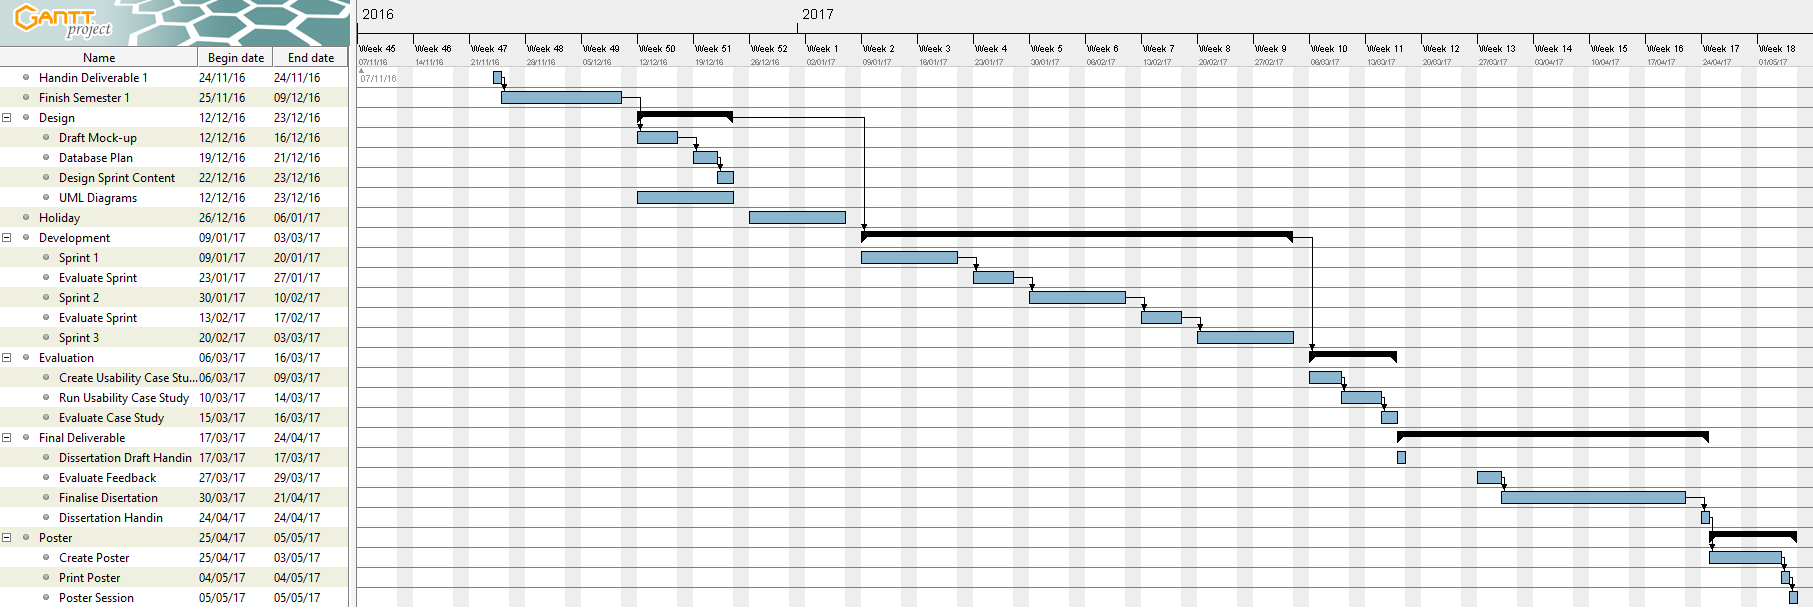
\includegraphics[width=\textwidth]{images/ganttchart.png}
\caption{Project Gantt Chart}
\label{fig:ganttchart}

\end{figure}




%%%%%%%%%%%%%%%%%%%%%%%%%%%%%%%%%%%%%%%%%
%										%
%     		Risk Analysis				%
%										%
%%%%%%%%%%%%%%%%%%%%%%%%%%%%%%%%%%%%%%%%%


\subsection{Risk Analysis}
\newcounter{risk} \stepcounter{risk}
The risks relating to this dissertation are shown in table(\ref{table:risk})


\begin{table}[h]

\caption{Risk Analysis}
\begin{tabular}{|p{0.05\textwidth}|p{0.25\textwidth}|p{0.15\textwidth}|p{0.1\textwidth}|p{0.33\textwidth}|}
\hline
\textbf{ID} & \textbf{Risk} & \textbf{Likelihood} & \textbf{Impact } & \textbf{Mitigation Strategy}
\\
\hline
+
R\arabic{risk} &Superviser Leaves & Low & Medium & Inform alisdair and request a new supervisor\\ \hline \stepcounter{risk}

R\arabic{risk} &Software Licenses Expire & Low & Low & Check licenses for all software i will be using during the project to make sure they are valid for length of project\\ \hline \stepcounter{risk}

R\arabic{risk} &Loss of data & Low & High & Back-ups will be stored throughout the project\\ \hline \stepcounter{risk}

R\arabic{risk} &Lecturers can’t create custom marking schemes & Medium & High\\ \hline \stepcounter{risk}

R\arabic{risk} &TRequirements changed & Medium & Medium & Evaluate requirements before starting development phase and evaluate requirements regularly during project to notice any required changes before it causes a major issue \\ \hline \stepcounter{risk}

R\arabic{risk} &System speed is slow & Medium & Medium\\ \hline \stepcounter{risk}

R\arabic{risk} &Users cannot understand the system & Medium & Medium\\ \hline \stepcounter{risk}

R\arabic{risk} &Browsers compatibility & High & High\\ \hline \stepcounter{risk}
R\arabic{risk} &Personal Injury & Low & High & Development would have to be delayed and discussions made with supervisor about how to continue\\ \hline \stepcounter{risk}
R\arabic{risk} &Test&Test&Test&test\\ \hline \stepcounter{risk}
R\arabic{risk} &Test&Test&Test&test\\ \hline










\end{tabular}
\label{table:risk}
\end{table}



%%%%%%%%%%%%%%%%%%%%%%%%%%%%%%%%%%%%%%%%%
%										%
%     			 P.L.E.S				%
%										%
%%%%%%%%%%%%%%%%%%%%%%%%%%%%%%%%%%%%%%%%%
\newpage

\subsection{Professional Issues}
The professional part of this project will be done by following coding standards for the languages that I decide to use.\\
As this project will be a Web application I will ensure that both the html and css are validated.\\
The system will be made open source to allow other people to look at and improve the system once I have completed it.\\
The project will be provided with a  user and developer documentation allow for easy development and implementation of the system.


\subsection{Legal Issues}
There are multiple legal issues relating to this project. The most important one is the Data Protection Act. Since the systems will be designed to store data about students I will have to make sure that all data is encrypted and securely stored.
I will make sure that any software included in the development of the system is open source and that I am meeting all the terms of service to use it.


\subsection{Ethical Issues}
A major ethical requirement of this project is to do with the storage of students personal information on a digital system; to deal with this issue I should consult the data protection act. \\
Another issue that is raised by this project is making sure that students are not deceived and that the marks they see are actually the ones they have received.


\subsection{Social Issues}
A few social issues are raised by this project. Such as if students can see the mark they have received straight away, will lab helpers feel pressurised into giving higher grades.\\
Will this system result in a reduction of lab helpers being required to mark labs? If the system speeds up the time to mark students’ work, less lab helpers may be required to run labs, resulting in people looking for work.



%%%%%%%%%%%%%%%%%%%%%%%%%%%%%%%%%%%%%%%%%
%										%
%     		Bibliography				%
%										%
%%%%%%%%%%%%%%%%%%%%%%%%%%%%%%%%%%%%%%%%%




\newpage
\bibliographystyle{plain}
\bibliography{references}




\end{document}